documentclass
\documentclass{article}
\usepackage{amsmath,amsfonts,bm}
\usepackage{xcolor}
\usepackage{tikz}
\usetikzlibrary{matrix}
\begin{document}

\begin{figure}[h]
    \centering
    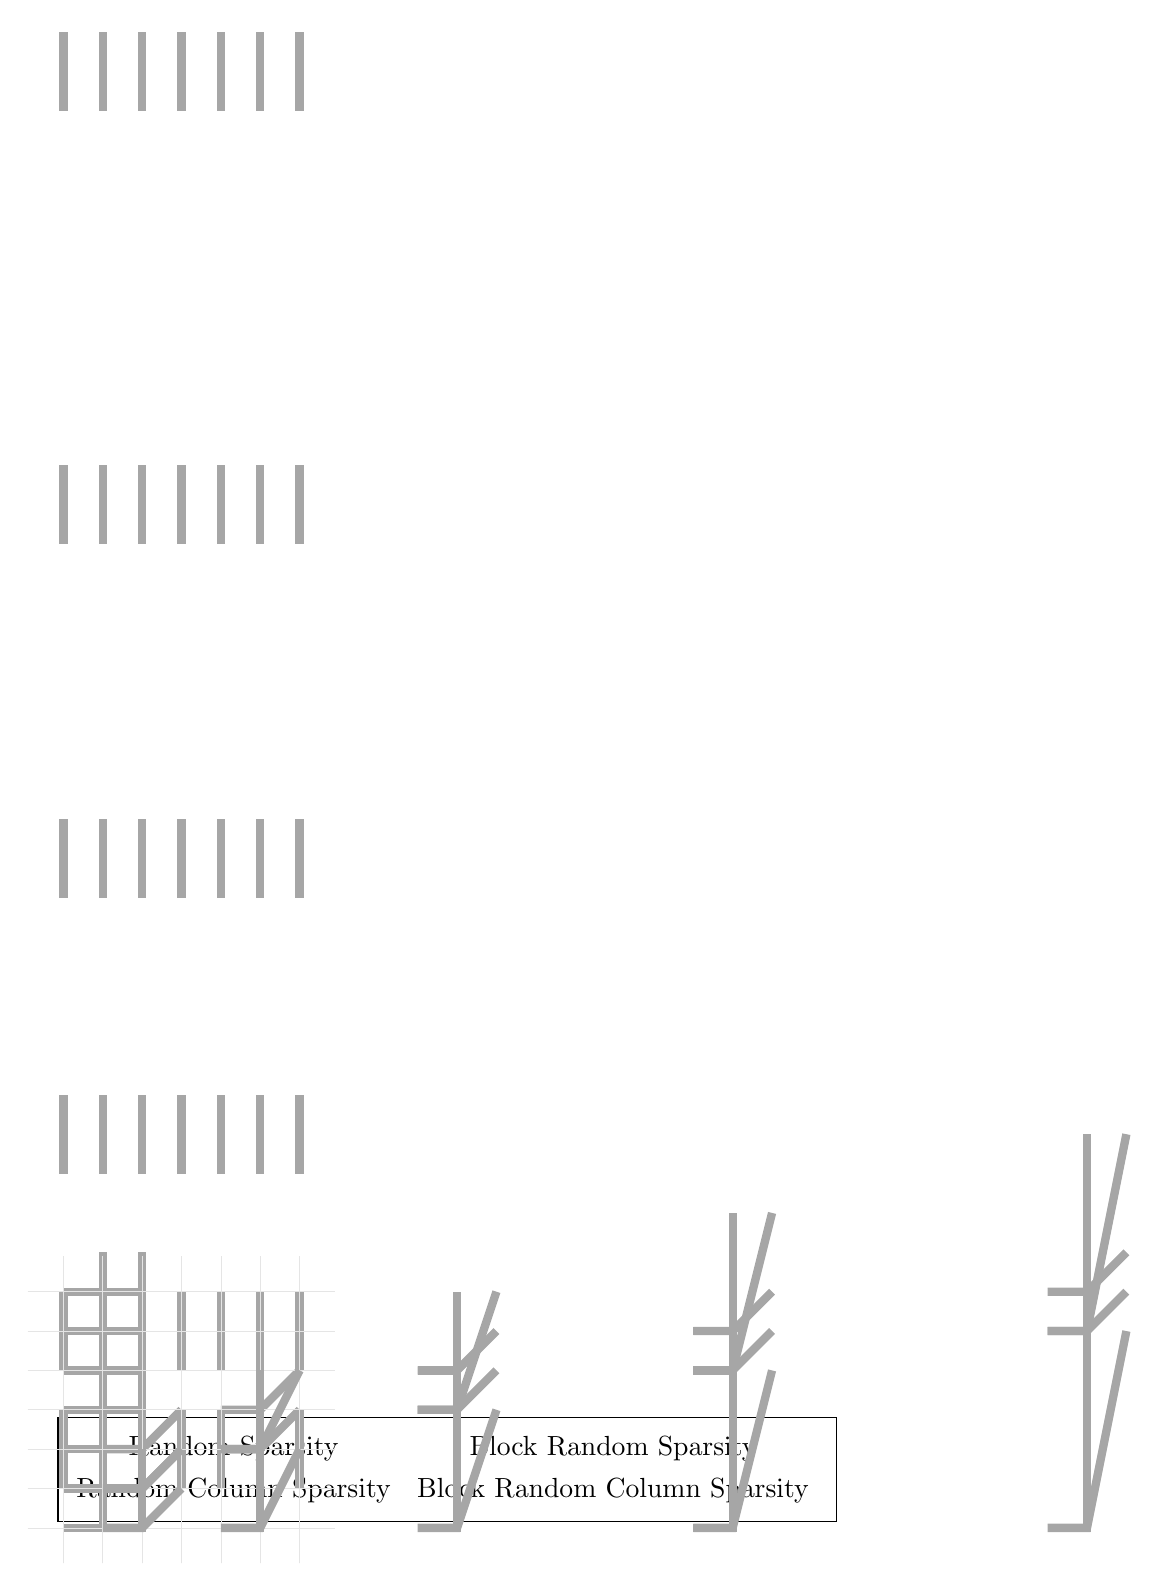
\begin{tikzpicture}[scale=0.5]
        \tikzset{mygrid/.style={draw,minimum width=1cm, minimum height=1cm}}
        \node[matrix, matrix of nodes, draw, anchor=south west, align=center, row sep=-\pgflinewidth, column sep=-\pgflinewidth] (mat) at (0,0){
            Random Sparsity & Block Random Sparsity \\
            Random Column Sparsity & Block Random Column Sparsity \\
        };
        \begin{scope}[yshift=-1ex, xshift=1ex]
            \draw[step=1cm,help lines, color=gray!20] (-0.9,-0.9) grid (6.9,6.9);
            \draw[line width=3pt, color=gray!70] (0,0) -- (1,0) -- (1,1);
            \draw[line width=3pt, color=gray!70] (1,0) -- (2,0) -- (2,1);
            \draw[line width=3pt, color=gray!70] (0,1) -- (1,1) -- (1,2);
            \draw[line width=3pt, color=gray!70] (1,1) -- (2,1) -- (2,2);
            \draw[line width=3pt, color=gray!70] (0,2) -- (1,2) -- (1,3);
            \draw[line width=3pt, color=gray!70] (1,2) -- (2,2) -- (2,3);
            \draw[line width=3pt, color=gray!70] (0,3) -- (1,3) -- (1,4);
            \draw[line width=3pt, color=gray!70] (1,3) -- (2,3) -- (2,4);
            \draw[line width=3pt, color=gray!70] (0,4) -- (1,4) -- (1,5);
            \draw[line width=3pt, color=gray!70] (1,4) -- (2,4) -- (2,5);
            \draw[line width=3pt, color=gray!70] (0,5) -- (1,5) -- (1,6);
            \draw[line width=3pt, color=gray!70] (1,5) -- (2,5) -- (2,6);
            \draw[line width=3pt, color=gray!70] (0,6) -- (1,6) -- (1,7);
            \draw[line width=3pt, color=gray!70] (1,6) -- (2,6) -- (2,7);
        \end{scope}
        \begin{scope}[yshift=-1ex, xshift=1ex]
            \draw[step=1cm,help lines, color=gray!20] (-0.9,-0.9) grid (6.9,6.9);
            \foreach \x in {1,...,5}{
                \draw[line width=3pt, color=gray!70] (\x*\x,\x) -- (\x*\x+1,\x) -- (\x*\x+1,\x+1);
                \draw[line width=3pt, color=gray!70] (\x*\x,\x) -- (\x*\x+1,\x) -- (\x*\x+2,\x+1);
                \draw[line width=3pt, color=gray!70] (\x*\x,\x+1) -- (\x*\x+1,\x+1) -- (\x*\x+1,\x+2);
                \draw[line width=3pt, color=gray!70] (\x*\x,\x+1) -- (\x*\x+1,\x+1) -- (\x*\x+2,\x+2);
            }
        \end{scope}
        \begin{scope}[yshift=-1ex, xshift=1ex]
            \draw[step=1cm,help lines, color=gray!20] (-0.9,-0.9) grid (6.9,6.9);
            \foreach \x in {1,...,6}{
                \draw[line width=3pt, color=gray!70] (0,\x*\x) -- (0,\x*\x+1) -- (0,\x*\x+2);
                \draw[line width=3pt, color=gray!70] (1,\x*\x) -- (1,\x*\x+1) -- (1,\x*\x+2);
                \draw[line width=3pt, color=gray!70] (2,\x*\x) -- (2,\x*\x+1) -- (2,\x*\x+2);
                \draw[line width=3pt, color=gray!70] (3,\x*\x) -- (3,\x*\x+1) -- (3,\x*\x+2);
                \draw[line width=3pt, color=gray!70] (4,\x*\x) -- (4,\x*\x+1) -- (4,\x*\x+2);
                \draw[line width=3pt, color=gray!70] (5,\x*\x) -- (5,\x*\x+1) -- (5,\x*\x+2);
                \draw[line width=3pt, color=gray!70] (6,\x*\x) -- (6,\x*\x+1) -- (6,\x*\x+2);
            }
        \end{scope}
        \begin{scope}[yshift=-1ex, xshift=1ex]
            \draw[step=1cm,help lines, color=gray!20] (-0.9,-0.9) grid (6.9,6.9);
            \foreach \x in {1,...,5}{
                \draw[line width=3pt, color=gray!70] (\x*\x,0) -- (\x*\x+1,0) -- (\x*\x+1,0+\x);
                \draw[line width=3pt, color=gray!70] (\x*\x,0) -- (\x*\x+1,0) -- (\x*\x+2,0+\x);
                \draw[line width=3pt, color=gray!70] (\x*\x,0+\x) -- (\x*\x+1,0+\x) -- (\x*\x+1,0+2*\x);
                \draw[line width=3pt, color=gray!70] (\x*\x,0+\x) -- (\x*\x+1,0+\x) -- (\x*\x+2,0+2*\x);
            }
        \end{scope}
    \end{tikzpicture}
\end{figure}
\end{document}